\hypertarget{index_intro}{}\section{Introduction}\label{index_intro}
The \char`\"{}Wi-\/11 Machine\char`\"{} is a simple, 16-\/bit computer architecture. It has 8 general purpose registers, 3 condition code registers (CCRs), and a program counter (PC). The Wi-\/11 Simulator is meant to emulate its execution, as well as present the user with information regarding the state of the machine after each instruction is executed. However, before one can delve into the behind-\/the-\/scenes details, one must understand the environment. In particular, an understanding of the object file syntax and the interactions between the components used in this project is necessary.\hypertarget{index_syntax}{}\section{Object Files}\label{index_syntax}
\begin{DoxyParagraph}{}
The object files (ususally file\_\-name.o) that this simulator accepts are ascii text files with the following structure: \begin{DoxyItemize}
\item One \hyperlink{index_header}{Header Record} \item Several \hyperlink{index_text}{Text Records} \item One \hyperlink{index_end}{End Record}\end{DoxyItemize}

\end{DoxyParagraph}
\hypertarget{index_header}{}\subsection{The Header Record}\label{index_header}
\begin{DoxyParagraph}{}
The Header Record is a single line that prepares the system for the storing the instructions to come. 
\end{DoxyParagraph}
\begin{DoxyParagraph}{}
{\bfseries Components} \begin{DoxyItemize}
\item A capital 'H'. This designates that it is the Header Record. \item A 6 character \char`\"{}segment name\char`\"{} (anything will do). \item A 4-\/digit Hexadecimal value that corresponds to the \char`\"{}load address\char`\"{} of the program. Instructions can be written starting at this address. \item A second 4-\/digit Hexadecimal value that denotes the length of the program-\/load segment (the size of memory into which the instructions will be loaded). \end{DoxyItemize}

\end{DoxyParagraph}
\begin{DoxyParagraph}{}
{\bfseries At a glance:} There is an 'H', a segment name, the first location where instructions can be written, and the number of memory locations for instuctions.
\end{DoxyParagraph}
\hypertarget{index_text}{}\subsection{Text Records}\label{index_text}
\begin{DoxyParagraph}{}
Following the Header Record are serveral Text Records. Each Text Record corresponds to a single machine instruction and, like the header record, is on a single line. 
\end{DoxyParagraph}
\begin{DoxyParagraph}{}
{\bfseries Components} \begin{DoxyItemize}
\item A capital 'T'. This designates that it is a Text Record. \item A 4-\/digit hexadecimal value -\/-\/ The location in memory at which the instruction will be stored. \item A second 4-\/digit Hexadecimal value -\/-\/ The encoding of the instruction to be stored. \end{DoxyItemize}

\end{DoxyParagraph}
\begin{DoxyParagraph}{}
{\bfseries At a glance:} There is a 'T', the location to store the instruction, and the instruction itself.
\end{DoxyParagraph}
\hypertarget{index_end}{}\subsection{The End Record}\label{index_end}
\begin{DoxyParagraph}{}
The End Record is, as the name would suggest, the last line of the line. Its purpose is to denote the end of instructions to be written and to give an initial value for the PC.\par
\par
 
\end{DoxyParagraph}
\begin{DoxyParagraph}{}
{\bfseries Components} \begin{DoxyItemize}
\item The End Record begins with a capital 'E'.\par
 \item Next, and last, a 4-\/digit hexadecimal value to be put into the PC. \end{DoxyItemize}

\end{DoxyParagraph}
\begin{DoxyParagraph}{}
{\bfseries At a glance:} There is an 'E', and the location in memory from which the first instruction should be fetched.
\end{DoxyParagraph}
\hypertarget{index_Component}{}\section{Interaction}\label{index_Component}
The components described in this document are, for the most part, representative of the actual hardware components that would be present in the Wi-\/11 machine. The following section describes these components and their interactions. After that, a list of the \hyperlink{index_instructions}{instructions} that the Wi-\/11 can execute (along with their encodings) completes the introduction to this simulator. The rest of the document details the workings of each component and provides the reader with the knowledge necessary for altering, fixing, or even just understanding the code itself.\hypertarget{index_components}{}\subsection{Components}\label{index_components}
The Wi-\/11 Simulator uses 5 major components (for a visual, see interactions). The main function, however, is only aware of one: \hyperlink{classWi11}{Wi11}. It creates one \hyperlink{classWi11}{Wi11} object and uses it to parse object files, decode the instructions, and execute them. In order to perform these tasks it first creates \hyperlink{classLoader}{Loader}, \hyperlink{classMemory}{Memory}, \hyperlink{classDecoder}{Decoder}, and \hyperlink{classRegister}{Register} objects. The \hyperlink{classRegister}{Register} objects correspond all those mentioned in the \hyperlink{index_intro}{Introduction}, with the exception of the CCRs which are declared as their own entity.

\begin{DoxyNote}{Note}
The \hyperlink{classWord}{Word} class is not described below but nearly all transfers of data and mathematical operations are performed using (an) object(s) of this type.
\end{DoxyNote}
\hypertarget{index_loading}{}\subsubsection{Loading}\label{index_loading}
The \hyperlink{classLoader}{Loader} object, recieving a pointer to memory and a filename, creates an \hyperlink{classObjParser}{ObjParser} object (the fifth major component). The \hyperlink{classObjParser}{ObjParser} pulls the relevant data from the file and the \hyperlink{classLoader}{Loader} puts it into memory. After some input by the user is accepted (assuming the simulator is in debug mode), the \hyperlink{classWi11}{Wi11} is ready to begin executing instructions.\hypertarget{index_execution}{}\subsubsection{Executing}\label{index_execution}
The \hyperlink{classWi11}{Wi11} component executes instructions in a way very similar to how an actual Wi-\/11 machine would execute them. It first has the \hyperlink{classMemory}{Memory} object return the instruction referenced by the current value of the PC. After incrementing the PC, the raw instruction is given to the \hyperlink{classDecoder}{Decoder}. The \hyperlink{classDecoder}{Decoder} returns an \hyperlink{structInstruction}{Instruction} object that allows the \hyperlink{classWi11}{Wi11} to call one of its many private functions that correspond (one-\/to-\/one) to each kind of instruction. This process is then repeated until either the HALT trap code is found or the user-\/specified instruction limit is reached.


\begin{DoxyImage}
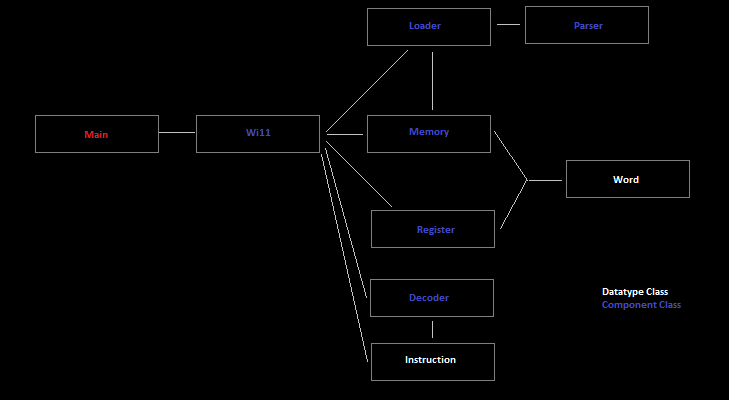
\includegraphics[width=\textwidth]{software_interaction.png}
\caption{This diagram shows the awareness of each component with those operating below it.}
\end{DoxyImage}
\hypertarget{index_instructions}{}\subsection{Wi-\/11 Instruction Set}\label{index_instructions}
